\problemname{Sopsug}
Grushög is an unfinished residential area in the outskirts of Lund. 
Right now, all necessary infrastructure is being constructed, including the most important
thing of all: garbage disposal. Like in many areas of Sweden, a \textit{sopsug} (automated vacuum collection 
system) will be used to collect garbage. The idea is to transport garbage underground through tubes using air pressure.

There are $N$ buildings in Grushög, numbered from $0$ to $N-1$. Your task is to connect some pairs
of buildings with tubes. If you build a tube from building $u$ to some other
building $v$, $u$ will send all of its garbage to $v$ (but not in the other direction). 
Your goal is to create a network of $N-1$ tubes such that all garbage ends up in one building.
In other words, you want the network to form a rooted tree, where the edges are directed toward the root.

However, $M$ tubes have already been constructed between buildings. These \textit{must} be used in your network. 
These tubes are directed, so they can only be used in one direction.

Furthermore, there are $K$ pairs of buildings between which it is impossible to build a tube. These pairs 
are ordered, so if it is impossible to build a tube from $u$ to $v$, it may still be possible to build
one from $v$ to $u$.

\section*{Input}

The first line of input contains the three integers, $N$, $M$, and $K$.

The following $M$ lines each contain two distinct integers $a_i, b_i$, meaning that 
there is already a tube from $a_i$ to $b_i$.

The following $K$ lines each contain two distinct integers $c_i, d_i$, meaning that 
it is impossible to build a tube from $c_i$ to $d_i$. 

All of the $M+K$ ordered pairs in the input will be distinct. 
Note that $(u,v)$ and $(v,u)$ are regarded as different pairs.

\section*{Output}

If there is no solution, print \texttt{NO}.

Otherwise, print $N-1$ lines, each containing two integers $u_i$, $v_i$, meaning that there should be 
a tube directed from $u_i$ to $v_i$.
You may print the tubes in any order. If there are multiple solutions, you may print any of them. 
Remember that all the $M$ already existing tubes must be included in your solution.

\section*{Constraints and Scoring}

\noindent
\begin{itemize}
  \item $2 \leq N \leq 300\,000$.
  \item $0 \leq M \leq 300\,000$.
  \item $0 \leq K \leq 300\,000$.
  \item $0 \leq a_i, b_i \leq N-1$ for $i = 0, 1, \ldots, M-1$.
  \item $0 \leq c_i, d_i \leq N-1$ for $i = 0, 1, \ldots, K-1$.
\end{itemize}

\noindent
Your solution will be tested on a set of test groups, each worth a number of points. 
Each test group contains a set of test cases. To get the points for a test group you need to 
solve all test cases in the test group.

\noindent
\begin{tabular}{| l | l | l |}
\hline
Group & Score & Limits \\ \hline
1     & 12    & $M = 0$ and $K = 1$  \\ \hline
2     & 10    & $M = 0$ and $K = 2$  \\ \hline
3     & 19    & $K = 0$  \\ \hline
4     & 13    & $N \leq 100$  \\ \hline
5     & 17    & It is guaranteed that there is a solution with $0$ as the root \\ \hline
6     & 11    & $M = 0$  \\ \hline
7     & 18    & No additional constraints  \\ \hline
\end{tabular}

\section*{Example}

The following figures show the first and second sample test cases.
The blue edges mark tubes which are already constructed, and the dashed red edges mark tubes which are impossible to build.

The figure to the left shows the first sample with the solution from the sample output, 
showing tubes with black edges (in addition to the already constructed tube from $4$ to $1$ which is blue).
In this network, all garbage will be collected in building $0$. 
This is not the only solution; for example, the tube from $1$ to $3$ can be replaced
by a tube from $0$ to $1$ and it is still a valid solution.

For the second sample input, we can see in the right figure that it is impossible to construct a solution
because of the cycle $(2, 3, 4)$.

\begin{center}
  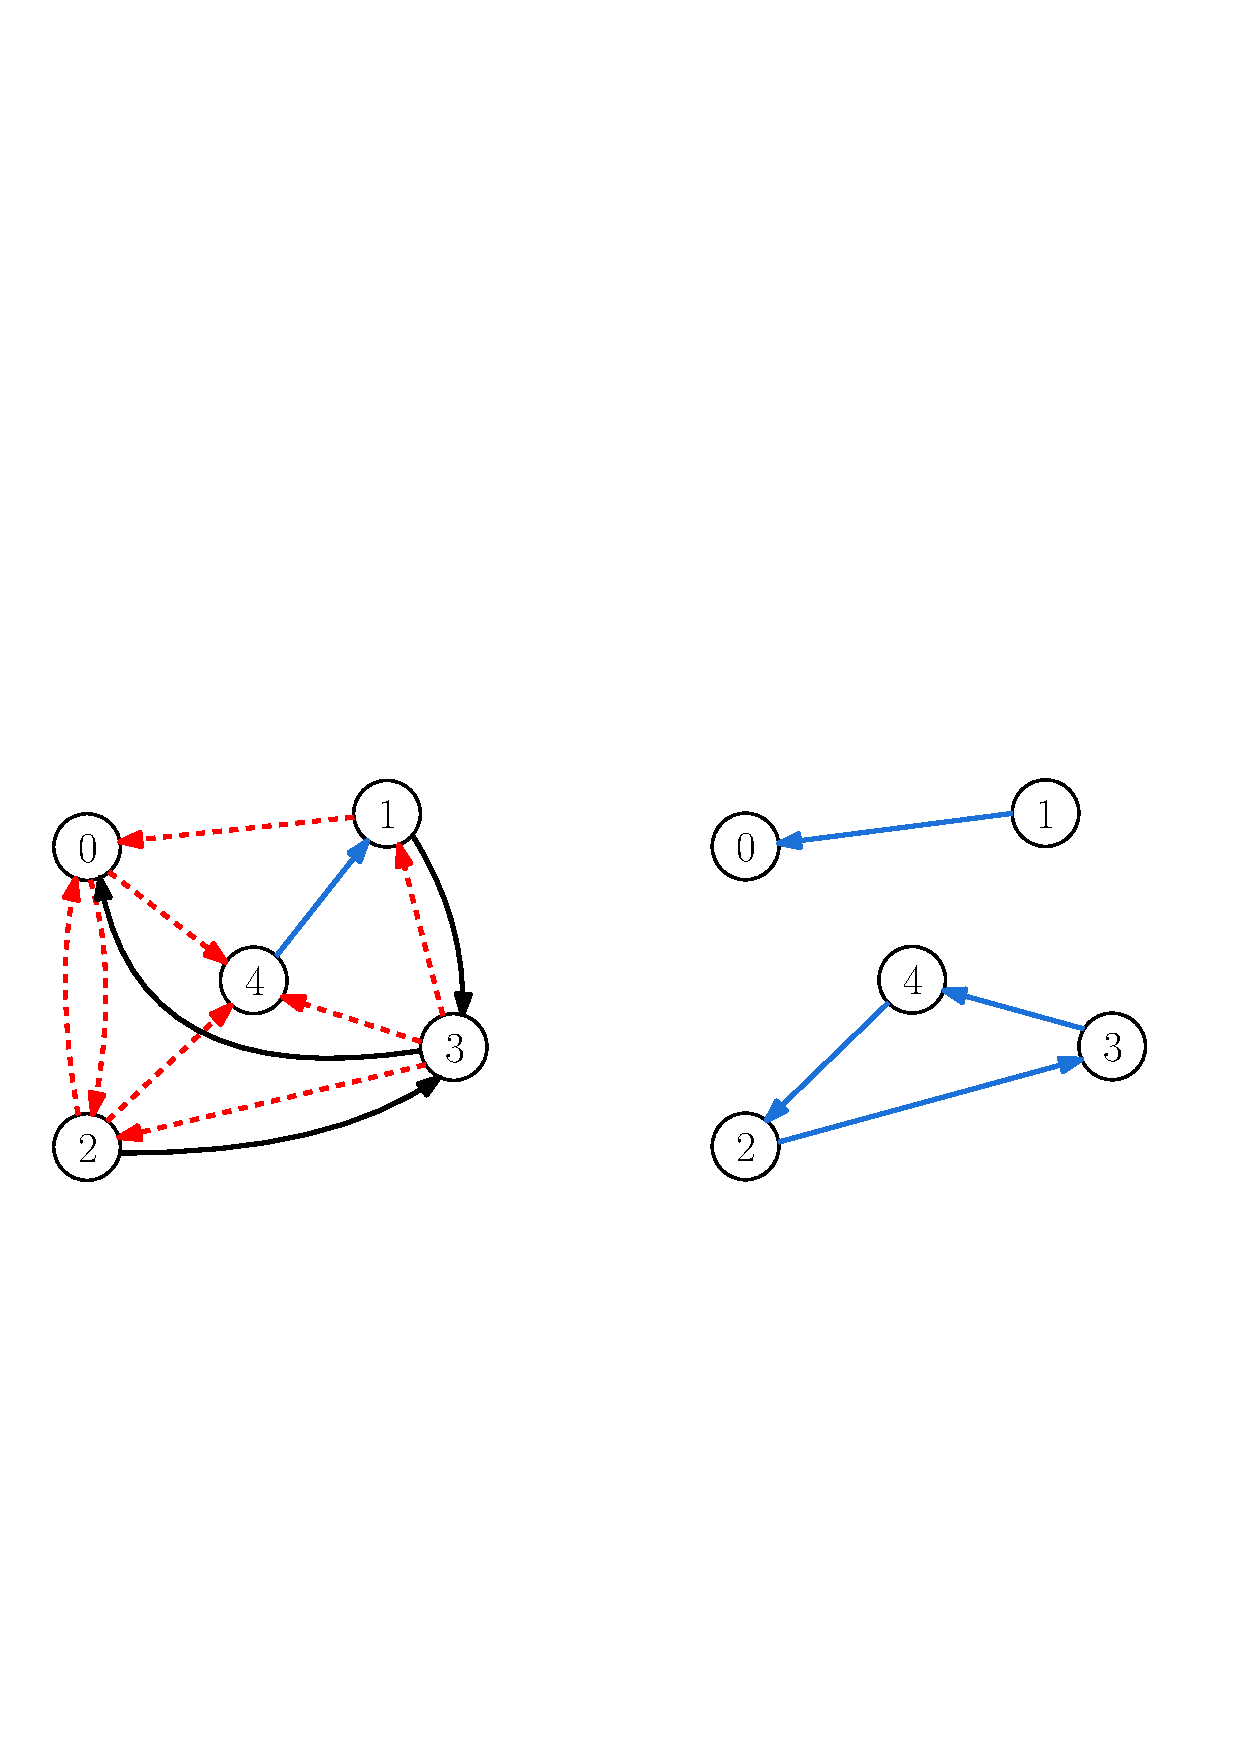
\includegraphics[width=.8\textwidth]{sample}
\end{center}

